\documentclass[]{article}

\usepackage{listings}
\usepackage{float}
\usepackage{graphicx}

\usepackage{titling}
\newcommand{\subtitle}[1]{%
  \posttitle{%
    \par\end{center}
    \begin{center}\large#1\end{center}
    \vskip0.5em}%
}

\begin{document}

\title{Lab 4: Simon}
\subtitle{CS M152A}
\author{Aman Agarwal \& Lowell Bander}

\maketitle
\tableofcontents

\newpage

\section{Introduction}
 
In this lab, we implemented an FPGA adaptation of the memory game, ``Simon". A sequence of LED's flashes in a particular order, after which the player inputs the sequence in the same order using the FPGA's switches. If successful, the user goes onto the next level which displays the same sequence of LEDs along with an additional, new random LED. \\

Additionally during the game, the seven segment display shows the current level that the user is on. The user can also play the game in a harder (faster) mode by flipping the difficulty switch.

\section{Design Description}

\subsection{High Level Design}
\begin{figure}[H]
\centering
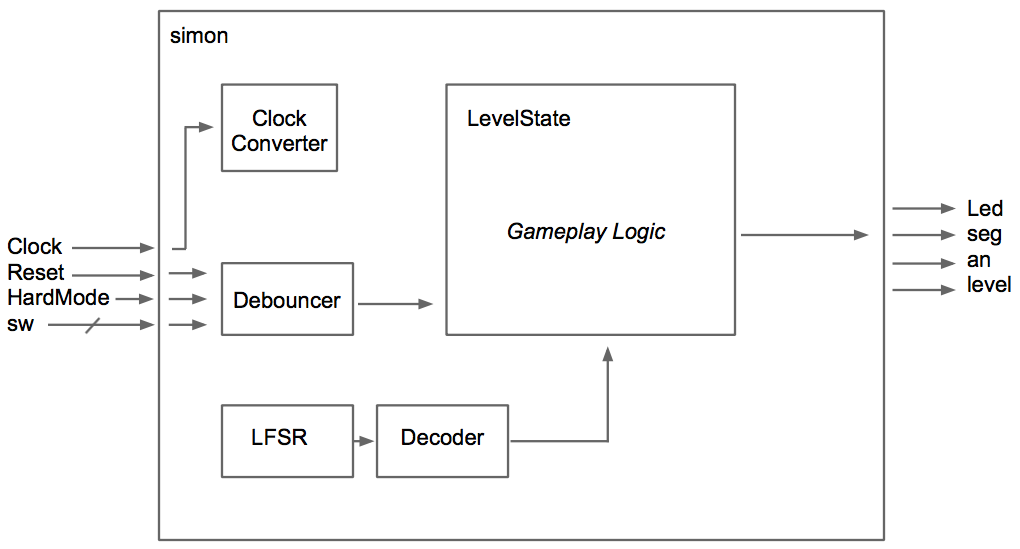
\includegraphics[width=\textwidth]{highLevel.png}
\caption{A high level diagram of our Simon game.}
\label{fig:high}
\end{figure}

As can be seen in the figure above, our top-level module accepts two main user inputs: \texttt{HardMode}, which indicates the difficulty level the user would enjoy, and \texttt{sw}, which represents the guesses the user makes during gameplay.\\

The \texttt{Led} output flashes lights above each switch to indicate to the user which of the four switches must be flipped during the level at hand. The \texttt{level} signal maps to the remaining 4 LEDs and shows the binary representation of the current level. Lastly, the \texttt{seg} and \texttt{an} outputs serve a similar purpose, except that they output the decimal representation of the current level.

\subsection{Low Level Implementation}
At a much smaller granularity, the our implementation of Simon proceeds as follows.\\

At setup, a random sequence is generated. The LFSR generates 2-bit random numbers one at a time, which are decoded to corresponding 4-bit values, and then shifted into a shift register. This operation halts when a counter reaches a preset value.\\

At this point, normal game logic proceeds. First, a single LED is flashed, instructing the user to flip the corresponding switch. If the user's input is incorrect, the game restarts. Alternatively, if the user's input is correct, the sequence of LEDs which are flashed is extended to contain 2 LEDs, and so on, until the user fails. The aforementioned validation is performed on every unit of user input, as opposed to validating the entire vector.\\

Throughout gameplay, the value of the current level is displayed in binary on the remaining four LEDs and is displayed in decimal on the 7 segment display.\\

All user input is routed through a debouncing unit before it arrives at the gameplay logic. This ensures that user input is only registered if it remains the same for at least 3 clock cycles.\\

Some functions, such as generating random numbers and validating user input can be performed using the very fast system clock, but other functions require a much slower clock. To accommodate this, a clock converter takes the system clock as input and outputs to slower clocks, the first of which is a 1 Hz clock which is used for flashing LEDs to the user. In the event that the \texttt{HardMode} signal is asserted, this signal is sped up to operate on a 2Hz clock. The other clock outputted by the converted module is much faster than the display clock but much slower than the system clock, and is used for the logic which controls the 7 segment display.

\section{Simulation Documentation}

Along with simulating and testing the overall game, we modularized our code and tested each of the modules individually. \\

For the overall game, we simulated the game from level one through level 10 and covered both correct and incorrect input. We discovered that when the user inputs an incorrect switch, the program did not produce a new random sequence but instead restarted the game using the same sequence from before. \\

Our simulation of the randomSequenceGenerator module showed that not only was our sequence ``pseudo-random", it had a period of 7 numbers. We then adjusted to increase that number.\\

We simulated both the easier and harder difficulties to see the differences.\\


\begin{figure}[H]
\centering
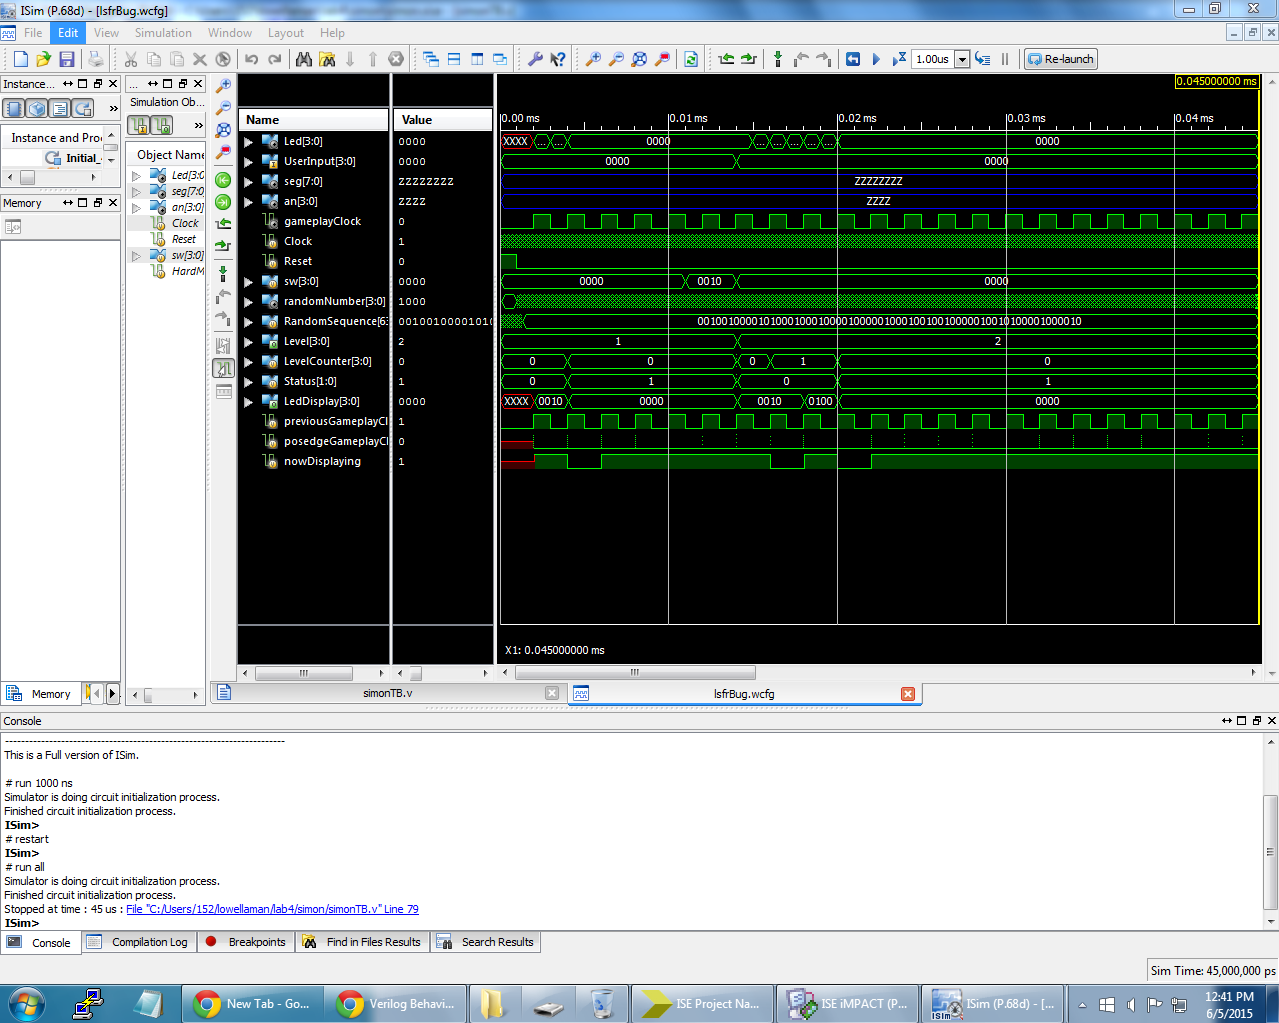
\includegraphics[width=\textwidth]{EasyMode.PNG}
\caption{Simulation of Simon in Easy mode.}
\label{fig:easy}
\end{figure}

\begin{figure}[H]
\centering
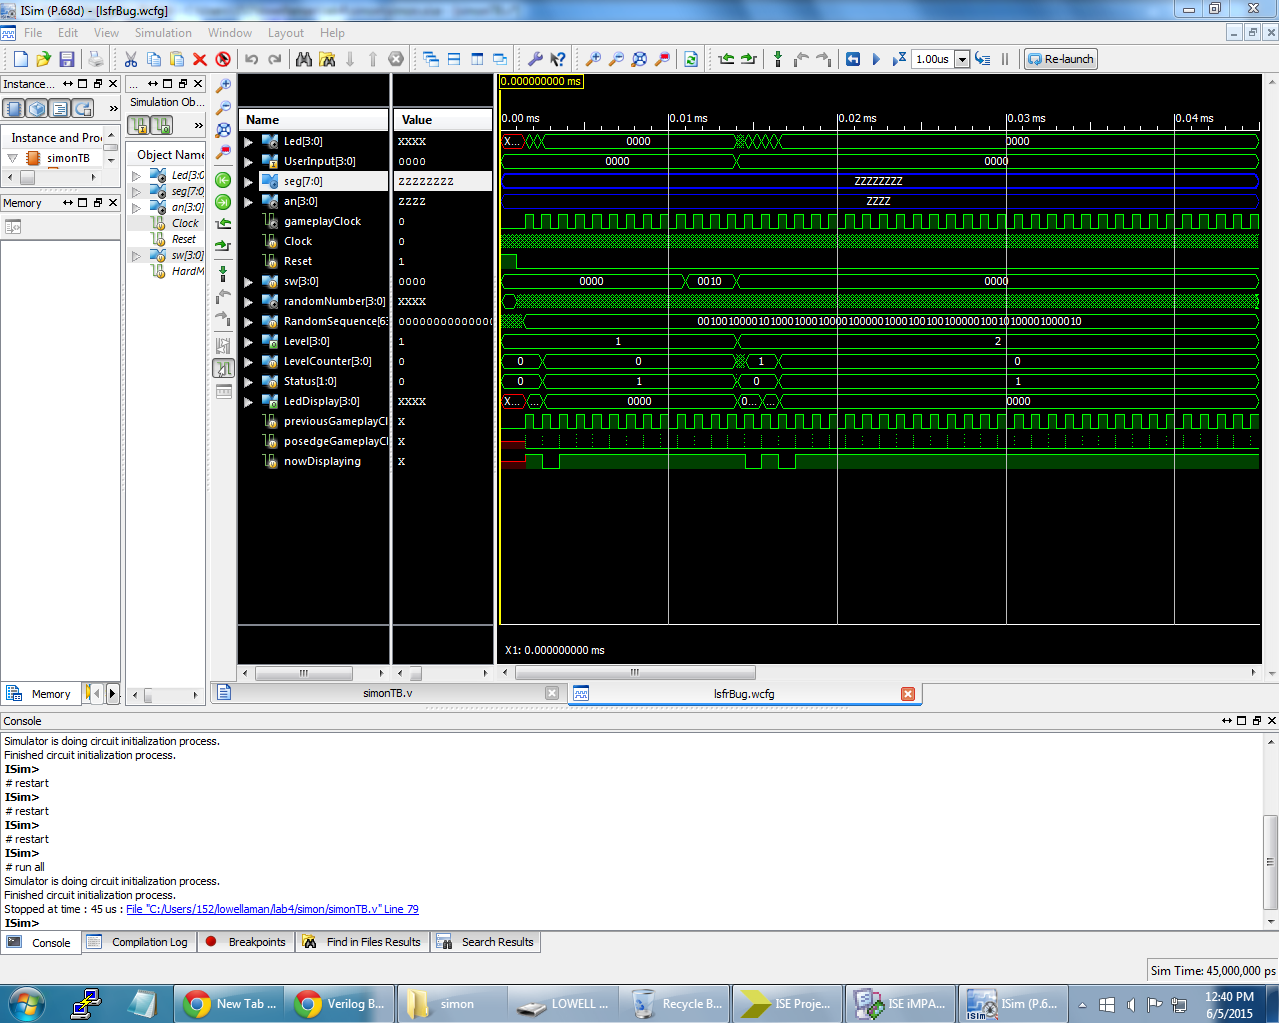
\includegraphics[width=\textwidth]{HardMode.PNG}
\caption{Simulation of Simon in Hard mode, twice the speed of Easy mode.}
\label{fig:hard}
\end{figure}

Because we had difficulties in Lab 3 with the Seven-Segment Display working properly, we simulated it. \\

\begin{figure}[H]
\centering
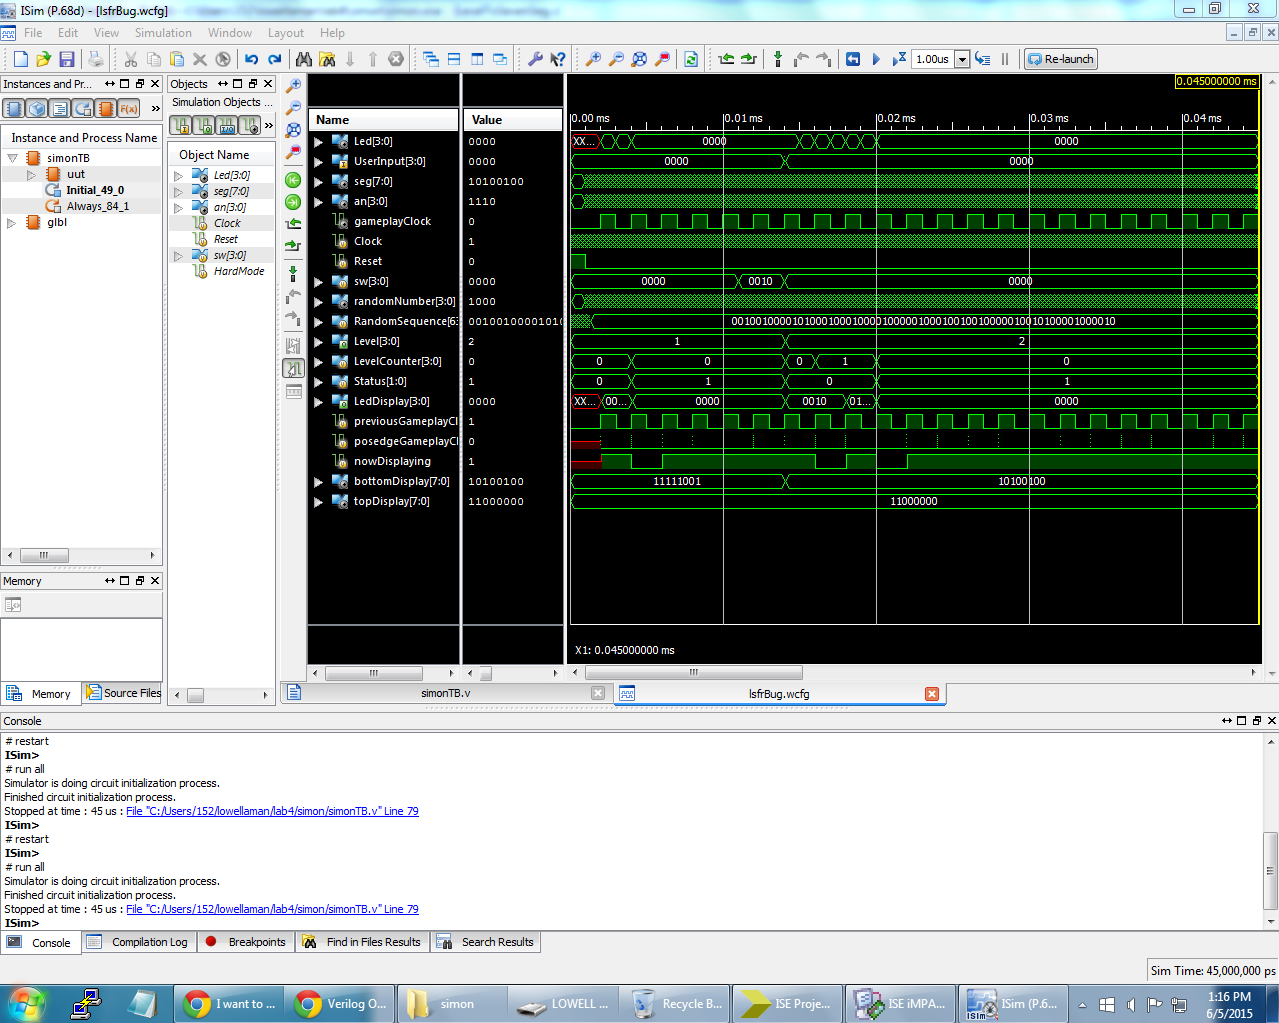
\includegraphics[width=\textwidth]{sevensegEasy.PNG}
\caption{The simulation of the seven segment display of the game in action.}
\label{fig:sevenseg}
\end{figure}


\section{Conclusion}
Being that this was our final project, we were able to learn from our mistakes from past projects. For our first project of this course, we made the mistake of writing all of our code in one big module and didn't test anything until we were done. In response to this, for our second project, we used very, very modular code fraught with good coding practices. Though this was aesthetically satisfying and avoided the problems encountered during our first project, the development process was too slow and as a result we were unable to finish our project before the deadline; that is to say, we would only have been able to see the fruit of our good coding practices were we to continue with the same codebase for several projects.\\

Using the above experience, the development process for our final project was a blend above the above approaches. This resulted in us being able to finish with a minimum viable product that demonstrated most of the functionality we set out to accomplish, and at the same time allowed us to iterate easily given the modular nature of our code.\\

In the end, the only bug in our code was that for every sequence of $n$ LED flashes, the first $n-1$ elements in the sequence flashed twice. Given the time remaining to complete the project, we decided to not attempt to fix this facet of our code base and instead spent our time implementing the remaining features.\\

Lastly, the only feature we failed to implement was `sound,' which in retrospect we should not have attributed such a sizable fraction of our project score to.



\end{document}

